% Dies ist Teil der Vorlesung Physik auf dem Computer, SS 2012,
% Axel Arnold, Universitaet Stuttgart.
% 
% Dieses Werk ist unter einer Creative Commons-Lizenz vom Typ
% Namensnennung-Weitergabe unter gleichen Bedingungen 3.0 Deutschland
% zugänglich. Um eine Kopie dieser Lizenz einzusehen, konsultieren Sie
% http://creativecommons.org/licenses/by-sa/3.0/de/ oder wenden Sie sich
% schriftlich an Creative Commons, 444 Castro Street, Suite 900, Mountain
% View, California, 94041, USA.

\chapter{Darstellung von Funktionen}

Auch moderne Prozessoren beherrschen nur die Grundrechenarten. Wie
kann man also auf einem Computer kompliziertere Funktionen berechnen,
wie z.B. die Sinusfunktion?

Beispielsweise könnte man die Funktionen als Vektor von
Funktionswerten speichern. Für die graphische Darstellung reicht das
aus, aber um Funktionen mit wenigstens sechs Stellen Genauigkeit im
Computer bereitzustellen, wären Millionen von Stützstellen nötig.

Daher müssen bessere Darstellungen für Funktionen genutzt werden.  Um
beliebige Funktionen auf dem Computer berechnen zu können, führt man
diese meist auf (stückweise definierte) Polynome zurück, die nur mit
Hilfe der Grundrechenarten berechnet werden können. Dies ist selbst
dann der Fall, wenn ein Prozessor gewisse Funktionen scheinbar in
Hardware implementiert hat; tatsächlich führt dieser intern die
notwendigen elementaren Operationen durch.

\section{\keyword{Horner-Schema}}
\label{sec:horner}

Die naive Auswertung eines Polynoms $\sum_{i=0}^{n} c_ix^{i}$ mit
$n+1$ Termen bzw. vom Grad $n$ benötigt $n$ Additionen und $2n$
Multiplikationen sowie einen Zwischenspeicher für die Potenzen $x^i$
des Arguments $x$. Besser ist die Auswertung des Polynoms nach dem
Horner-Schema:
\begin{equation}
  \label{eq:horner}
  \sum_{i=0}^{n} c_ix^{i} = c_0 + x(c_1 + x(c_2 + x(\ldots (c_{n-1} + x c_{n})))).
\end{equation}
Wird dieser Ausdruck von rechts nach links ausgewertet, so muss das
Ergebnis in jedem Schritt nur mit $x$ multipliziert und der nächste
Koeffizient addiert werden, was nur $n$ Multiplikationen und
Additionen benötigt. Auch muss kein Zwischenwert gespeichert werden,
was Prozessorregister spart. Als C-Code sieht die Auswertung des
Hornerschemas so aus:
\begin{lstlisting}[language=C]
double horner(double *series, int n, double x)
{
    double r = c[n];
    for(int i = n-1; i >= 0; --i)
        r = r*x + c[i];
    return r;
}
\end{lstlisting}
\sloppypar Die Polynomauswertung stellt NumPy als
\scipy{numpy.polyval(x, c)} zur Verfügung. \argd{c} bezeichnet die
Koeffizienten des Polynoms und \argd{x} das Argument, für das das
Polynom ausgewertet werden soll.

Eine weitere Anwendung des Hornerschemas ist die Polynomdivision durch
lineare Polynome der Form $x-x_0$, die zum Beispiel wichtig für die
iterative Bestimmung von Nullstellen ist. Es gilt nämlich
\begin{equation}
  \label{eq:polynomdiv}
  P(x) = \sum_{i=0}^{n} c_ix^{i} = 
  \left(\sum_{i=0}^{n-1} d_{i+1}x^{i}\right)(x-x_0) + d_0,
\end{equation}
wobei $d_i = c_i + x_0(c_{i+1} + x_0(\ldots (c_{n-1} + x_o c_n)))$ die
Zwischenterme des Hornerschemas bei Auswertung an der Stelle $x_0$
sind. $d_0$ ist dabei der Divisionsrest; ist $P(x)$ durch $x-x_0$
teilbar, so ist $d_0=0$. 

Dies zeigt man durch Induktion: für $P(x) = c_1 x + c_0$ ist offenbar
$P(x) = c_1(x-x_0) + c_0 + x c_1 = d_1(x-x_0) + d_0$. Für Grad $n$ ist
also
\begin{equation}
    P(x) = x \left(\sum_{i=0}^{n-1} c_{i+1}x^{i}\right) + c_0
    = x\left(\sum_{i=0}^{n-2} d'_{i+1}x^{i}(x-x_0) + d'_0\right) +
    d_0
\end{equation}
wobei sich die $d'_i = c_{i+1} + x_0(c_{i+2} + x_0(\ldots (c_{n-1} +
x_o c_n))) = d_{i+1}$ bei der Polynomdivision von $\sum_{i=0}^{n-1}
c_{i+1}x^{i}$ durch $x-x_0$ ergeben. Daher ist
\begin{equation}
    P(x) = \left(\sum_{i=0}^{n-2} d_{i+2}x^{i+1} + d_1\right)(x-x_0) +
    d_0 + x_0 d_1,
\end{equation}
was zu zeigen war.

\section{Taylorreihen}
\index{Taylorreihe}

\begin{figure}
  \centering
  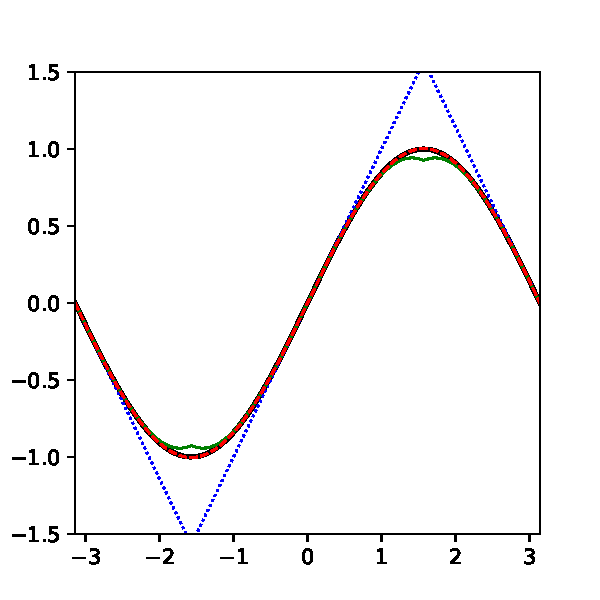
\includegraphics[width=0.5\textwidth]{plots/sinus}
  \caption{Näherung der Sinusfunktion durch die abgeschnittene
    Taylorreihe. Als schwarze durchgezogene Linie ist die tatsächliche
    Sinusfunktion dargestellt, blau gepunktet ist die Näherung erster
    Ordnung um Null, $x$, grün durchgezogen ist die kubische Näherung
    $x - x^3/6$, und rot gestrichelt $x-x^3/6 + x^5/120$. Die Kurven
    nutzen die Symmetrie der Sinuskurve, sind also an $\pm\pi/2$
    gespiegelt.}
  \label{fig:sinus}
\end{figure}

Nachdem wir nun wissen, wie Polynome effizient ausgewertet werden
können, stellt sich die Frage, wie man ein gutes Näherungspolynom für
eine Funktion bekommt. Dazu gibt es viele verschiedene Ansätze, deren
Vor- und Nachteile im Folgenden kurz besprochen werden. Der älteste
Ansatz, der auch in der Analytik weiten Einsatz findet, ist die
Taylorentwicklung.  Ist eine Funktion $f$ um einen Punkt $x_o$
hinreichend gut differenzierbar, lässt sie sich als bekannterweise
lokal als Taylorreihe darstellen:
\begin{equation}
  f(x) = \sum_{i=0}^\infty \frac{f^{(i)}(x_0)}{i!} (x-x_0)^i,
  \label{eq:taylor}
\end{equation}
wobei $f^{(i)}(x)$ die $i$-te Ableitung von $f$ an der Stelle $x$
bezeichnet.  Falls die Ableitungen existieren und $x-x_0$ klein genug
ist, so konvergiert diese Darstellung schnell, und einige Terme
genügen, um zufriedenstellende Genauigkeit zu erreichen. Lokal um den
Entwicklungspunkt $x_0$ is eine abgeschnittene Taylorreihe also eine
gute polynomielle Näherung. Leider gibt es für die meisten Funktionen
einen Konvergenzradius, außerhalb dessen die Reihe nicht einmal
konvergiert. Daher eignen sich Taylorreihen vor allem gut für kleine
Umgebungen. Auch ist eine abgeschnittene Taylorreihe nur im
Entwicklungspunkt $x_0$ exakt; dort stimmen allerdings gleich die
ersten $i$ Ableitungen.

Um  zum  Beispiel die  oben  angeführte  Sinusfunktion  mit 7  Stellen
Genauigkeit im Interval $[0:\pi/2]$  auszuwerten, genügen die ersten 7
Terme der Taylorreihe. Mit Hilfe der Symmetrien der Funktion lässt sie
sich damit bereits für alle Argumente auswerten. Da
\begin{equation*}
  \sin'(x) = \cos(x) \quad\text{und} \quad \cos'(x) = -\sin(x),
\end{equation*}
ergibt sich die bekannte Reihe
\begin{equation}
  \sin(x) = \sum_{i=0}^\infty \frac{\sin^{(i)}(0)}{i!} x^i =
  \sum_{i=0}^\infty \frac{(-1)^i}{(2i+1)!} x^{2i+1}.
\end{equation}
Wie gut diese Darstellung mit entsprechender Rückfaltung funktioniert,
zeigt Abbildung~\ref{fig:sinus}.  Für viele andere komplexe Funktionen
ist es ebenfalls möglich, Taylorreihen analytisch oder numerisch zu
bestimmen, die dann zur Auswertung auf dem Computer genutzt werden
können.

\section{Polynom- oder Lagrangeinterpolation}
\index{Interpolation}
\index{Interpolation>Polynom-}
\index{Interpolation>Lagrange-}

\begin{figure}
  \centering
  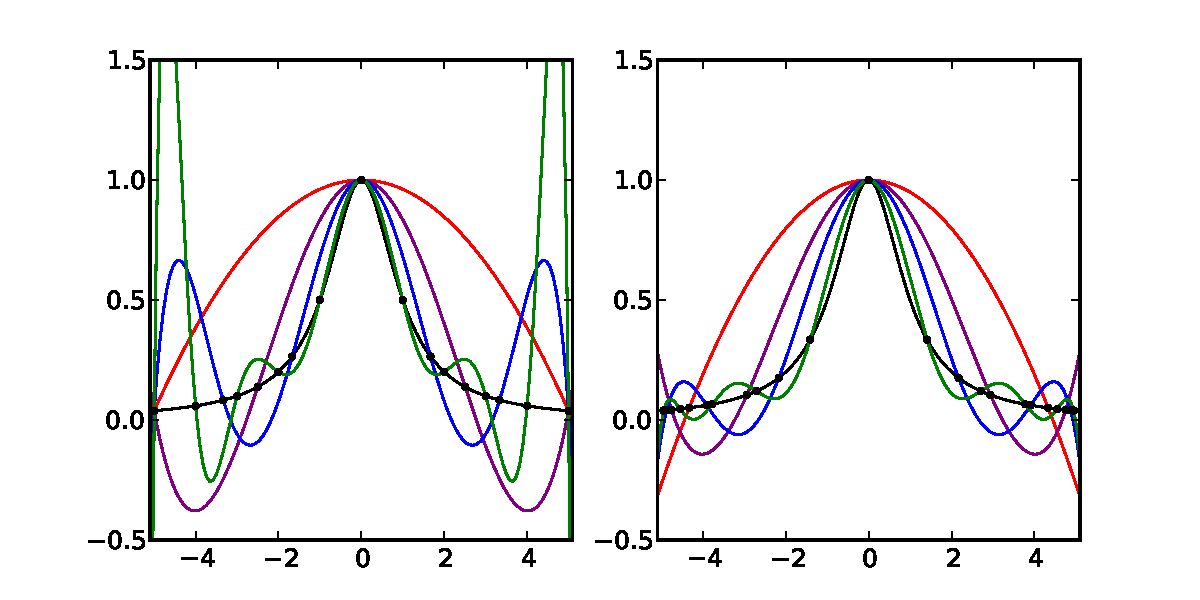
\includegraphics[width=\textwidth]{plots/runge_lagrange}
  \caption{Lagrange-Interpolation der Rungefunktion $1/(1+x^2)$
    (schwarze Linie). Im linken Graph sind die Stützstellen
    äquidistant gewählt (markierte Punkte), die farbigen Linien sind
    die interpolierenden Polynome durch 3 (rot), 5 (lila), 7 (blau)
    und 11 (grün) Stützstellen. Mit steigender Ordnung wird die
    Interpolation am Rand immer schlechter, das Polynom 10. Ordnung
    erreicht Werte bis nahe an zwei. Im rechten Graph sind
    für die gleichen Ordnungen Chebyshev-Stützstellen gewählt worden,
    die den Interpolationsfehler minimieren.}
  \label{fig:runge}
\end{figure}

Wie besprochen ist eine abgeschnittene Taylorreihe nur im
Entwicklungspunkt exakt (dann allerdings auch die Ableitungen),
innerhalb des Konvergenzradius nur eine Annäherung, und außerhalb des
Konvergenzradius sogar divergent.  Oft möchte man aber eher für einen
größeren Wertebereich eine gute (oder wenn möglich exakte) Darstellung
der Funktion haben.

Eine Möglichkeit dazu bietet die Polynom- oder
Lagrangeinterpolation. Dazu legt man eine Anzahl von Punkten im
gewünschten Wertebereich fest (die sogenannten \emph{Stützstellen}).
Wie sich zeigt, gibt es dann genau ein Polynom, dass die Funktion an
diesen Punkten exakt interpoliert. Genauer: seien Punkte $(x_i, y_i)$,
$i=0(1)n-1$ gegeben mit $x_i$ paarweise verschieden. Dann gibt es
genau ein Polynom $P(x)=\sum_{k=0}^{n-1} a_kx^{k}$ vom Grad $n-1$, so
dass $P(x_i) = y_i$, da die Gleichung
\begin{equation}
  \begin{split}
    y_1 &= P(x_0) = a_0 + a_1 x_0 + \cdots + a_{n-1}x_0^{n-1}\\
    \vdots\\
    y_n &= P(x_{n-1}) = a_0 + a_1 x_{n-1} + \cdots + a_{n-1}x_{n-1}^{n-1}
  \end{split}
  \label{eq:interpol}
\end{equation}
genau eine Lösung hat.

Leider ist aber nicht gewährleistet, dass mit steigender Anzahl von
Punkten die Funktion auch zwischen den Stützstellen immer besser
angenähert wird. Tatsächlich hat Runge ein einfaches Beispiel
angegeben, nämlich die Rungefunktion $1/(1+x^2)$, für die die Näherung
mit steigender Anzahl an äquidistanten Punkten immer schlechter wird,
siehe Abbildung~\ref{fig:runge}.

Bei der etwas allgemeineren Hermite-Interpolation können an den
Stützstellen neben den Funktionswerten auch Ableitungen vorgegeben
werden. Das eindeutige interpolierende Polynom hat dann einen Grad,
der der Gesamtanzahl an vorgegebenen Funktionswerten und Ableitungen
entspricht. Ist zum Beispiel nur eine Stützstelle $x_0$ gegeben und
neben dem Funktionswert $n$ Ableitungen, so entspricht das
Hermite-Polynom genau den ersten $n+1$ Termen der Taylorreihe.

Das interpolierende Polynom kann nicht nur zur Interpolation verwendet
werden, also der Bestimmung an Punkten zwischen den Stützstellen,
sondern --- mit Vorsicht --- auch zur Extrapolation, also um Werte
außerhalb des Bereichs zu bestimmen. Da bei der Hermite-Interpolation
auch die Ableitungen insbesondere am Rand kontrolliert werden können,
ist diese hier tendenziell vorteilhafter. Extrapolation spielt eine
wichtige Rolle, wenn eine direkte Auswertung der Zielfunktion
numerisch zu teuer oder unmöglich wird. Bei Computersimulationen tritt
dies insbesondere in der Nähe von kritischen Punkten auf.

In SciPy liefert die Funktion \scipy{scipy.interpolate.lagrange(x, y)}
das interpolierende Polynom durch die Stützstellen (\argd{x[i]},
\argd{y[i]}).

\subsection{\keyword{Lagrangepolynome}}

Die Koeffiziente $a_i$ können im Prinzip als Lösung von
Gleichung~\eqref{eq:interpol} mit geeigneten Lösern für lineare
Gleichungssysteme gefunden werden, was im allgemeinen allerdings recht
langsam ist. Daher benutzt man besser eine direkte Darstellung mit
Hilfe der \emph{Lagrangepolynome}, die wie folgt definiert sind:
\begin{equation}
  \label{eq:lagrange}
  L_i(x) = \prod_{k\neq i} \frac{x-x_k}{x_i-x_k}.
\end{equation}
Die Polynominterpolation wird daher auch Lagrange-Interpolation
genannt.  Wie man leicht sieht, gilt $L_i(x_k) = \delta_{ik}$, so dass
das Polynom\index{interpolierendes Polynom>Lagrangedarstellung}
\begin{equation}
  P(x) = \sum_{i=1}^n y_i\,L_i(x)
\end{equation}
das eindeutige interpolierende Polynom durch $(x_i, y_i)$
ist.

Diese Darstellung ist allerdings für praktische Zwecke nur sinnvoll,
wenn sich die Stützstellen $x_i$ nicht ändern, da die Bestimmung der
Lagrangepolynome $L_i(x)$ zeitaufwändig ist. Geeigneter ist die
\emph{baryzentrische Darstellung} \index{interpolierendes
  Polynom>baryzentrische Darstellung}
\begin{equation}
P(x) = \sum_{i=0}^{n-1} y_i\, \mu_i \; \Big/ \; \sum_{i=0}^{n-1}
\mu_i\quad\text{mit}\quad
\mu_i := \frac{1}{x-x_i}\prod_{k\neq i}\frac{1}{x_i-x_k},
\end{equation}
bei der lediglich der Quotient zweier rationaler Funktionen gebildet
werden muss. 

\subsection{\keyword{Neville-Aitken-Schema}}

Das rekursive Neville-Schema ist eine effiziente Möglichkeit, das
interpolierende Polynom auszuwerten ohne es tatsächlich zu
berechnen. Das ist nützlich, wenn nur wenige Auswertungen nötig sind,
wie zum Beispiel beim Romberg-Integrationsverfahren, bei dem zur
Schrittweite 0 extrapoliert wird.

Wir definieren $P_{i,k}$ als das interpolierende Polynom der Ordnung
$k-1$ durch die Stützstellen $x_j, j=i(1)i+k-1$.  Gesucht ist der Wert
$P(x)=P_{0,n}(x)$ des interpolierenden Polynoms an der Stelle $x$.
Dann ist
\begin{align}
  P_{i,1}(x)&=y_i \quad\text{für}\, i=0(1)n-1
  \intertext{und}
  \label{eq:divdiff}
  P_{i,k}(x)&= \frac{P_{i,k-1}(x)(x_{i+k-1} - x) + P_{i+1,k-1}(x)(x -
    x_i)}{x_{i+k-1} - x_i} \quad\text{für}\, k=2(1)n, i=0(1)n-k,
\end{align}
da ja an den inneren Stützstellen $x_l$, $l=i+1(1)i+k-2$,
$P_{i,k-1}(x_l)=P_{i+1,k-1}(x_l) = y_l$ gilt, und per Konstruktion
$P_{i,k}(x_i)=y_i$ und $P_{i,k}(x_{i+k-1})=y_{i+k-1}$. Durch
sukzessives Berechnen zunächst der $P_{i,2}(x)$, dann der
$P_{i,3}(x)$, usw. lässt sich das interpolierende Polynom bequem an
einer fixen Stelle auswerten. Als (Neville-)Schema sieht das so aus:
\begin{center}
  \begin{tikzpicture}[on grid=true, node distance=1.5em and 10em]
    \node (u01) {$y_0$};
    \node[below=of u01] (u11) {$y_1$};
    \node[below=of u11] (u21) {$y_2$};
    \node[below=of u21] (u31) {$y_3$};
    \node[below=of u31] (u41) {$\vdots$};
  
    \node[right=of u11] (u02) {$P_{0,2}(x)$};
    \node[below=of u02] (u12) {$P_{1,2}(x)$};
    \node[below=of u12] (u22) {$P_{2,2}(x)$};
    \node[below=of u22] (u32) {$\vdots$};
  
    \node[right=of u12] (u03) {$P_{0,3}(x)$};
    \node[below=of u03] (u13) {$P_{1,3}(x)$};
    \node[below=of u13] (u23) {$\vdots$};

    \node[right=of u13] (u04) {$P_{0,3}(x)$};
    \node[below=of u04] (u14) {$\vdots$};

    \draw[->] (u01) -- (u02);
    \draw[->] (u11) -- (u02);
    \draw[->] (u11) -- (u12);
    \draw[->] (u21) -- (u12);
    \draw[->] (u21) -- (u22);
    \draw[->] (u31) -- (u22);

    \draw[->] (u02) -- (u03);
    \draw[->] (u12) -- (u03);
    \draw[->] (u12) -- (u13);
    \draw[->] (u22) -- (u13);

    \draw[->] (u03) -- (u04);
    \draw[->] (u13) -- (u04);
  \end{tikzpicture}
\end{center}
wobei die Pfeilpaare dividierte Differenzen gemäß \eqref{eq:divdiff} bedeuten.

\subsection{Newtonsche Darstellung}
\index{interpolierendes Polynom>Newtonsche Darstellung}

Wir betrachten nun die Polynome $P_{0,k}$ des Nevilleschemas. Es gilt
offenbar
\begin{equation}
  P_{0,k}(x) - P_{0,k-1}(x) = \gamma_k(x-x_0)\cdots(x-x_{k-2}),
\end{equation}
da die beiden Polynome in den Stützstellen $x_0,\ldots,x_{k-2}$
übereinstimmen und die Differenz ein Polynom vom Grad $k-1$ ist, also
höchstens $k-1$ Nullstellen hat. Weiter ist $\gamma_k$ der führende
Koeffizient des Polynoms $P_{0,k}(t)$, da $P_{0,k-1}(t)$ ja einen
niedrigeren Grad hat. Daraus ergibt sich die folgende \emph{Newtonsche
  Darstellung} des interpolierenden Polynoms:
\begin{equation}
  \begin{split}
    P_{0,n}(x) &= y_0 + \sum_{k=2}^{n} P_{0,k}(x) - P_{0,k-1}(x)\\
    &= y_0 + \gamma_2(x-x_0) + \gamma_3(x-x_0)(x-x_1) + \cdots
    + \gamma_n(x-x_0)\cdots(x-x_{n-2})\\
    &= y_0 + (x-x_0)\biggl(\gamma_2 + (x-x_1)\Bigl(\gamma_3 + \cdots
    \bigl(\gamma_{n-1} + (x-x_{n-2})\gamma_n\bigr)\cdots\Bigr)\biggr).
  \end{split}
\end{equation}
Die letztere Umformung zeigt, dass sich die Newtonsche Darstellung
effizient mit einem leicht abgewandelten Hornerschema auswerten lässt:
\begin{lstlisting}
def horner(x0, x, gamma):
    r = 0
    for k in range(len(x)-1, -1, -1):
        r = r*(x0-x[k]) + gamma[k];
    return r
\end{lstlisting}

Die Koeffizienten $\gamma_i$, $i=2(1)n$ lassen sich dabei bequem mit
dem Nevilleschema bestimmen. $\gamma_k$ ist ja der höchste Koeffizient
von $P_{0,k}$ ist, der sich leicht aus \eqref{eq:divdiff} berechnen
lässt. Wenn $\gamma_{i,k}$ den führenden Koeffizienten des Polynoms
$P_{i,k}$ bezeichnet, so erhalten wir das Nevilleschema
\begin{align}
  \gamma_{i,1} &= y_i \quad\text{für}\, i=0(1)n-1\quad\text{und}\\
  \gamma_{i,k}&= \frac{\gamma_{i+1,k-1} - \gamma_{i,k-1}}{x_{i+k-1} -
    x_i}
  \quad\text{für}\, k=2(1)n, i=0(1)n-k.
\end{align}
Da letztlich nur die $\gamma_{0,k}$ interessant sind, also die obere
Diagonale des Nevilleschemas, benötigt man für die Berechnung nur
einen Vektor
\begin{equation}
  \gamma' = \left(\gamma_{0,1},\gamma_{0,2},\ldots,\gamma_{0,k-1},
    \gamma_{0,k},\gamma_{1,k},\ldots,\gamma_{n-k,k}\right),
\end{equation}
der wie folgt berechnet wird:
\begin{lstlisting}
def neville(x, y):
    n = len(x)
    gamma = y.copy()
    for k in range(1, n):
        for i in range(n-k-1, -1, -1):
            gamma[i+k] = (gamma[i+k] - gamma[i+k-1])/(x[i+k] - x[i])
    return gamma
\end{lstlisting}
Man beachte, dass die Schleife über $i$ herunterläuft, um benötigte
Werte nicht zu überschreiben.

\subsection{\keyword{Chebyshev-Stützstellen}}

Bis jetzt haben wir wenig zur Wahl der Stützstellen gesagt. Oft liegt
es auch nahe, äquidistante Stützstellen zu verwenden wie im
Fadenpendel-Beispiel. Man kann allerdings zeigen, dass die
Chebychev-Stützstellen den Fehler der Polynominterpolation minimieren.
Diese sind definiert als die Nullstellen der Polynome (!)
\begin{equation}
  T_n(\cos\phi) = \cos(n\phi),
\end{equation}
die offensichtlich zwischen -1 und 1 liegen und daher geeignet
skaliert werden müssen für die Interpolation in einem allgemeinen
Interval. Die Chebychev-Polynome $T_n$, $n\ge 0$, bilden eine
orthogonale Basis der Funktionen über $[-1,1]$ bezüglich des mit
$1/\sqrt{1-x^2}$ gewichteten Skalarprodukts. Daher kann jede genügend
glatte Funktion auf $[-1:1]$ als eine Reihe
\begin{equation}
  f(x) = \sum_{n=0}^\infty a_n T_n(x)
\end{equation}
dargestellt werden, die sogenannte Chebyshev-Reihe (siehe auch z.B.
\textcite{abramowitz70a}).

 Explizit sind diese Nullstellen gegeben durch
\begin{equation}
  x_{k,n} = \cos\left(\frac{2k+1}{2n}\pi\right),\quad k=0(1)n-1.
\end{equation}
Wird die Rungefunktion mit Chebyshevstützstellen interpoliert, so
konvergiert das interpolierende Polynom, im Gegensatz zu äquidistanten
Stützstellen.

\section{Splines}
\index{Spline}
\index{Interpolation>Spline-}

Wie wir gesehen haben, kann unter ungünstigen Umständen die Güte der
Polynominterpolation mit steigender Anzahl an Stützstellen sinken, vor
allem, wenn diese äquidistant verteilt sind. Oft ist das aber nicht zu
vermeiden, zum Beispiel, wenn die Daten in einem Experiment regelmäßig
gemessen werden. Das Problem ist, das die Koeffizienten des Polynoms
global gelten, sich glatte Funktionen aber nur lokal wie ein Polynom
verhalten (Taylorentwicklung!). Daher ist es günstiger, statt der
gesamten Funktion nur kleine Abschnitte durch Polynome zu nähern.

Der einfachste Fall einer solchen Näherung ist die \emph{lineare
  Interpolation}\index{Interpolation>lineare}, bei der die
Stützstellen durch Geraden, also Polynome vom Grad 1, verbunden
werden. Sind die Stützstellen $(x_i, y_i)$, $i=1(1)n$ gegeben, so ist
der lineare interpolierende Spline
\begin{equation}
  P_1(x) = \frac{(x_{i+1} - x)y_i + (x - x_i)y_{i+1}}
  {x_{i+1}-x_i}
  \quad\text{für}\, x_i \le x < x_{i+1}.
\end{equation}

\begin{figure}
  \centering
  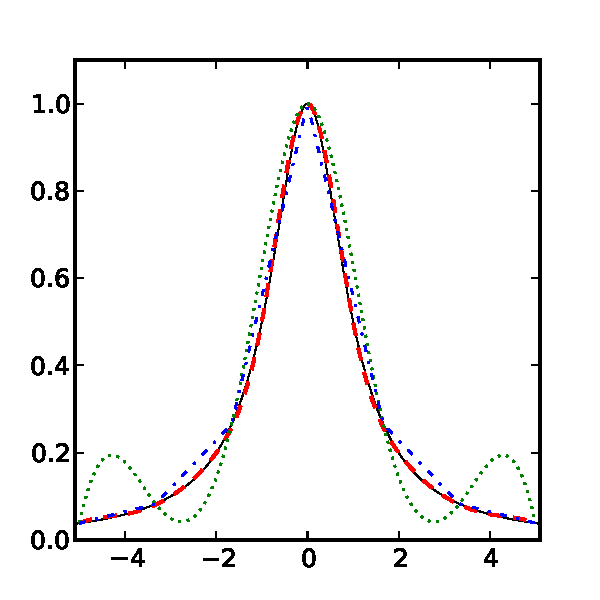
\includegraphics[width=0.5\textwidth]{plots/splines}
  \caption{Spline-Interpolation der Rungefunktion (durchgezogene
    schwarze Linie). Die gestrichelte blaue Linie ist die lineare
    Spline-Interpolierende mit 7 Stützstellen, die anderen Kurven sind
    kubische Splines mit 7 (grün gepunktet) und 11 Stützstellen (rot
    gestrichelt). Mit 11 Stützstellen ist der Spline von der
    Rungefunktion praktisch nicht mehr zu unterscheiden.}
  \label{fig:spline}
\end{figure}

Diese Funktionen sind aber an den Stützstellen im allgemeinen nicht
differenzierbar. Soll die Interpolierende differenzierbar sein, müssen
Polynome höherer Ordnung genutzt werden. Solche stückweise definierten
Polynome heißen \emph{Splines} --- das englische Wort Splines
bezeichnete dünne Latten, die vor dem Computerzeitalter benutzt
wurden, um glatte, gebogene Oberflächen vor allem für Schiffsrümpfe zu
entwickeln. Der wichtigste Spline ist der \emph{kubische} oder
\emph{natürliche}
Spline\index{Spline>kubisch}\index{Spline>natürlich}, der aus
Polynomen dritten Grades zusammengesetzt und zweifach stetig
differenzierbar ist. Seine allgemeine Form ist
\begin{equation}
  P_3(x) = y_i + m_i(x-x_i) + \frac{1}{2}M_i(x-x_i)^2 + \frac{1}{6}\alpha_i(x-x_i)^3
  \quad\text{für}\, x_i \le x < x_{i+1}.
\end{equation}
Da die zwei rechten und linken zweiten Ableitungen an den Stützstellen
übereinstimmen müssen, gilt
\begin{equation}
  \alpha_i = \frac{M_{i+1} - M_i}{x_{i+1} - x_i}.
\end{equation}
Aus der Gleichheit der Funktionswerte an den Stützstellen ergibt sich
\begin{equation}
  m_i = \frac{y_{i+1} - y_i}{x_{i+1}-x_i} -
  \frac{1}{6}(x_{i+1}-x_i)(2M_i + M_{i+1}).
\end{equation}
Aus der Gleichheit der ersten Ableitungen ergibt sich schliesslich ein
Gleichungssystem für die $M_i$. Hier kommen in den Gleichungen
gleichzeitig $M_{i-1}$, $M_i$ und $M_{i+1}$ vor, daher müssen für die
Randwerte weitere Vorgaben gemacht werden. Sollen die Splines am Rand
festgelegte 2. Ableitungen $M_0$ und $M_n$ haben, so hat das
Gleichungssystem die Form
\begin{equation}
  \label{eq:spline1}
  \begin{pmatrix}
    2      & \lambda_1 &           &           &           &         0 \\
    \mu_2  & 2         & \lambda_2 \\
           &           & \ddots    & \ddots    & \ddots \\
           &           &           & \mu_{n-2}  & 2         & \lambda_{n-2} \\
    0      &           &           &           & \mu_{n-1}  & 2         \\
  \end{pmatrix}
  \begin{pmatrix}
    M_1\\
    M_2\\
    \vdots\\
    M_{n-2}\\
    M_{n-1}
  \end{pmatrix} \,=\,
  \begin{pmatrix}
    6S_1 - \mu_1 M_0\\
    6S_2\\
    \vdots\\
    6S_{n-2} \\
    6S_{n-1} -  \lambda_{n-1} M_n
  \end{pmatrix},
\end{equation}
mit
\begin{equation}
  \lambda_i = \frac{x_i - x_{i-1}}{x_{i+1} - x_{i-1}},\quad
  \mu_i = \frac{x_{i+1}-x_i}{x_{i+1} + x_{i-1}}\quad\text{und}\quad
  S_i = \frac{\frac{y_{i+1}-y_i}{x_{i+1} -
      x_i} - \frac{y_i-y_{i-1}}{x_i - x_{i-1}}}{x_{i+1}-x_{i-1}}.
\end{equation}
Auch periodische Funktionen können kubisch interpoliert werden, wobei
dann die zusätzliche Bedingungen durch die Kontinuität über die periodische
Grenze hinweg gegeben sind. Die Gleichungen für $\alpha_i$ und $m_i$
sind dabei unverändert, nur das Gleichungssystem wird
\begin{equation}
  \label{eq:spline2}
  \begin{pmatrix}
    2      & \lambda_1 &           &           &           &      \mu_1 \\
    \mu_2  & 2         & \lambda_2 &           & 0\\
           &           & \ddots    & \ddots    & \ddots \\
           & 0          &           & \mu_{n-2}  & 2         & \lambda_{n-2} \\
    \lambda_{n-1} &           &           &           & \mu_{n-1}  & 2         \\
  \end{pmatrix}
  \begin{pmatrix}
    M_1\\
    M_2\\
    \vdots\\
    M_{n-2}\\
    M_{n-1}
  \end{pmatrix} \,=\,
  \begin{pmatrix}
    6S_1\\
    6S_2\\
    \vdots\\
    6S_{n-2} \\
    6S_{n-1}
  \end{pmatrix},
\end{equation}
wobei die Funktion als $x_n-x_1$-periodisch mit $y_1=y_n$
vorausgesetzt wird. Abbildung~\ref{fig:spline} zeigt die
Spline-Interpolation der Rungefunktion, die für diesen
Interpolationstyp keine Probleme zeigt.

Die Gleichungssysteme \eqref{eq:spline1} und \eqref{eq:spline2} sind
sehr gut konditioniert und mit einem einfachen Gleichungslöser zu
behandeln.  Zum Beispiel ist die Gauß-Elimination ist für die hier
auftretenden einfachen Bandstrukturen sehr effizient. In SciPy gibt es
selbstverständlich bereits eine fertige Routine für die
Spline-Interpolation, nämlich \scipy{scipy.interpolate.interp1d(x, y,
  kind)}. (\argd{x},\argd{y}) sind dabei die Stützstellen, und
\argd{kind} eine Zeichenkette, die den Typ des Splines
bestimmt. Mögliche Werte sind zum Beispiel "`linear"' und "`cubic"'
für lineare bzw. kubische interpolierende Splines.

\section{Ausgleichsrechnung, Methode der kleinsten Quadrate}
\index{Ausgleichsrechnung}
\index{Fitting}
\index{Methode der kleinsten Quadrate}

\begin{figure}
  \centering
  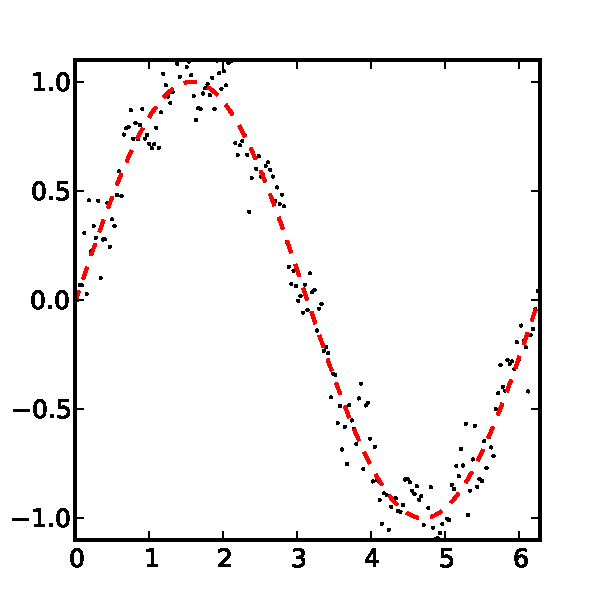
\includegraphics[width=0.5\textwidth]{plots/leastsq}
  \caption{Methode der kleinsten Quadrate zum Fitten der Sinusfunktion
    $y=\sin(x)$. 200 Datenpunkte zwischen 0 und $2\pi$ wurden als
    $\sin(x) + 0,1\,\sin(10 x) + \xi$ erzeugt, wobei $\xi$ eine
    Gauß-verteilte Pseudozufallsvariable mit Varianz $0,01$ war. Die
    resultierende Sinusfunktion (rot gestrichelt) hat die Form $a
    \sin(bx+c)$, wobei die Koeffizienten auf gut 2\% Genauigkeit
    $a=b=1$ und $c=0$ entsprechen. Die kleine höherfrequente
    Schwingung kann durch einen Fit allerdings nicht zuverlässig
    erkannt werden.}
  \label{fig:leastsq}
\end{figure}

Interpolierende Polynome, Taylorreihen und Splines haben gemeinsam,
das diese exakt durch die gegebenen Stützstellen verlaufen. Oftmals
ist das aber gar nicht gewünscht, da die Daten selbst nicht exakt
sind, zum Beispiel wenn diese aus einem Experiment oder einer
Simulation stammen. In diesem Fall hat man üblicherweise eine
Vorstellung, welche funktionelle Form die Daten annehmen, und möchte
nun wissen, mit welchen Parametern diese Funktion am besten mit den
Daten verträglich ist. Dazu muss man den Parametersatz bestimmen, so
dass der Abstand der Daten von der Funktion minimiert wird.

Seien also wieder Daten $(x_i, y_i)$, $i=1(1)n$ und eine Funktion
$f_v(x)$ gegeben. Gesucht ist dann derjenige Parametervektor $v$, der
die Abweichung
\begin{equation}
  \label{eq:leastsq}
  \Delta(v) = \sum_i (f_v(x_i) - y_i)^2
\end{equation}
minimiert. Dieses Verfahren wird auch Methode der kleinste Quadrate
genannt, da ja die quadrierten Abweichungen minimiert werden
sollen. Ist $f_{a,b}(x) = ax + b$ eine Gerade, spricht man auch von
\emph{linearer Regression}\index{lineare Regression}. In diesem Fall lässt
sich das Optimum einfach bestimmen, da
\begin{equation}
  0 = \frac{d}{da} \Delta(a,b) = \sum_i 2 (a x_i + b - y_i)x_i
  = 2N \left(a  \left<x_i^2\right> + b \left<x_i\right> -
    \left<y_ix_i\right> \right)
\end{equation}
und
\begin{equation}
  0 = \frac{d}{db} \Delta(a,b) = \sum_i 2 (a x_i + b - y_i)
  = 2N \left(a  \left<x_i\right> + b - \left<y_i\right> \right),
\end{equation}
wobei $\left<\cdot\right>$ den Mittelwert über alle Datenpunkte
bedeutet. Daraus ergibt sich
\begin{equation}
  a = \frac{\left<y_ix_i\right> -
    \left<y_i\right>\left<x_i\right>}{\left<x_i^2\right>-\left<x_i\right>^2}
  \quad\text{und}\;
  b = \left<y_i\right> - a \left<x_i\right>,
\end{equation}
was sich einfach auf dem Computer berechnen lässt.

Auch für quadratische und andere einfache Funktionen lassen sich die
Koeffizienten geschlossen darstellen, aber bei allgemeinen Funktionen
ist dies nicht immer der Fall. Dann muss die nichtlineare
Optimierungsaufgabe \eqref{eq:leastsq} numerisch gelöst werden, was
wir später behandeln werden. Für den Moment genügt uns, dass SciPy die
Funktion \scipy{scipy.optimize.leastsq(delta, v0, (x, y))} dafür
bereitstellt. \argd{(x, y)} sind dabei die Ausgangsdaten, die hier zu
einem Tupel zusammengefasst sind. \argd{v0} ist der Startwert für die
Berechnung, der nicht zu weit vom (unbekannten) Optimum entfernt
liegen darf. \argd{delta} ist eine Python-Funktion, die als Argumente
$v$, $x_i$ und $y_i$ nimmt und $f_v(x_i) - y_i$ zurückliefert.  Da
$f_v(x)$ eine beliebig komplizierte Form annehmen kann, ist diese
Aufgaben im allgemeinen nicht lösbar, allerdings funktioniert ein
solcher \emph{Fit} für einfache Funktionen meistens recht
gut. Abbildung~\ref{fig:leastsq} zeigt einen solchen Funktionsfit an
eine verrauschte Sinusfunktion, die mit 200 Datenpunkten auf etwa 2\%
genau gefittet werden kann. Man beachte, das der Ausgangswert für den
Fit mit Hilfe der SciPy-Funktion \lstinline!leastsq! $a=0$, $b=1$,
$c=0$ war; beim Startwert $a=0$, $b=0$, $c=0$ bricht das Verfahren
ab. Das zeigt, dass man tatsächlich nicht zu weit vom Optimum starten
kann, was ein gewisses Verständnis der Zielfunktion voraussetzt.

Ist die Funktionsform, die den Daten zugrundeliegt, unbekannt, ist es
normalerweise keine gute Idee, die Form zu raten. Generell sollte auch
die Anzahl der Parameter sehr klein sein, da sich sonst fast alles
"`gut"' fitten lässt ("`With four parameters I can fit an elephant and
with five I can make him wiggle his trunk."' --- J. von Neumann).

Soll aber zum Beispiel für Visualisierungszwecke eine ansprechende
Kurve entlang der Daten gelegt werden, deren tatsächliche Abhängigkeit
unbekannt ist, dann sind \emph{Pad\'e-Funktionen} oft eine gute
Wahl. Diese haben die Gestalt $P(x)/Q(x)$, wobei $P$ und $Q$ zwei
Polynome mit paarweise verschiedenen Nullstellen sind. Üblicherweise
lassen sich schon niedrigen Polynomgraden ansprechende Fits finden,
sofern die Grade der beiden Polynome in etwa gleich gewählt werden.

\section{Fourierreihen}

Bis jetzt waren unsere Näherungsfunktionen auf Polynomen basierend, da
diese einerseits vom Computer verarbeitet werden können und
andererseits aufgrund der Taylorentwicklung glatte Funktionen meist
gut approximieren. Für periodische Funktionen sind Polynome aber an
sich erst einmal wenig geeignet, da sie selbst nicht periodisch
sind. Splines können zwar auch periodisch gemacht werden, aber
trotzdem sind trigonometrische Funktionen besser geeignet, um
periodische Funktionen darzustellen. Fourierreihen und
-transformationen stellen Funktionen als trigonometrische Reihen dar,
die meist gut konvergieren und darüberhinaus einige nützliche
Eigenschaften haben.

Es gibt zwei Hauptanwendungen der Fourierdarstellung: die Analyse und
Aufbereitung periodischer Signale und die Lösung von
Differentialgleichungen.  Bei periodischen Signalen dient die
Fourierdarstellung zur Analyse des \emph{Spektrums} des Signals.
Diese gibt nützliche Informationen über die charakteristischen
Zeitskalen von Strukturen im Signal, zum Beispiel die Tonhöhe und die
Obertonreihe eines Instruments. In dieser Frequenzdarstellung lassen
sich auch gezielt einzelne Frequenzen dämpfen, was Rauschen
unterdrücken kann und im ursprünglichen Funktionsraum teure Faltungen
erfordert.  Bei Differentialgleichungen nutzt man aus, dass die
Ableitung im Frequenzraum eine algebraische Operation ist, und die
Differentialgleichung somit in eine gewöhnliche algebraische (und oft
sogar lineare) übergeht.

\subsection{Komplexe Fourierreihen}
\index{Fourierreihen>komplexe}
\index{Fouriertransformation>komplexe}
Wir betrachten eine periodische Funktion $f(t)$ mit $f(t+T) = f(t)$
für alle $t\in\RR$, d.h. $f$ hat Periode $T$. Dann ist die
Fourierdarstellung von $f$ gegeben durch
\begin{equation}
  \label{eq:fourier}
  f(t) = \sum_{n\in\ZZ} \hat{f}_n e^{i n\omega t}
\end{equation}
mit $\omega=2\pi/T$. Die Koeffizienten $\hat{f}_n$ lassen sich
berechnen als
\begin{equation*}
  \label{eq:fouriercoeff}
  \hat{f}_n = \frac{1}{T}\int_0^T f(t)e^{-i n\omega t}\, dt
\end{equation*}
und sind im allgemeinen komplex, auch wenn $f$ reellwertig ist. Die
Beiträge $\hat{f}_{\pm n}$ haben dieselbe Frequenz $\pm n/T$,
unterscheiden sich aber in ihrer Phase. Die \emph{Leistung} zu dieser
Frequenz ist $\hat{f}_{n}\hat{f}_{-n}$.

\eqref{eq:fourier} lässt sich auch so lesen, dass
\begin{equation}
  e^{-i n\omega t} = \cos(n \omega t) + i \sin(n \omega t)
\end{equation}
eine orthonormale Basis bezüglich des Skalarprodukts
\begin{equation}
  \label{eq:l2scalar}
  (f, g) = \frac{1}{T}\int_0^T f(t)\overline{g(t)}\,dt
\end{equation}
bilden. Ähnlich wie ein Vektor im $\RR^n$ wird die Funktion $f$ also
durch die Fouriertransformation in ihre Schwingungskomponenten
zerlegt.  Insbesondere sind die Fourierkoeffizienten linear in der
Funktion, d.h.
\begin{equation}
  \widehat{f+\lambda g}_n = \hat{f}_n +\lambda \hat{g}_n.
\end{equation}

Die Voraussetzungen für die Konvergenz der Fourierreihe sind sehr
schwach - solange die Funktion wenigstens quadratintegrabel ist,
konvergiert die Fourierreihe fast überall, d.h.
\begin{equation}
  \left\lVert f(t) - \sum_{n=-N}^N \hat{f}_n e^{i n\omega t} \right\rVert \xrightarrow{N\to\infty} 0.
\end{equation}
Daneben ist die Transformation $f\to\hat{f}$ eine \emph{Isometrie},
genauer gilt das \emph{\keyword{Parsevaltheorem}}
\begin{equation}
  \sum_{n\in\ZZ} \lvert\hat{f}_n\rvert^2 =
  \frac{1}{\omega}\int_0^t \lvert f(t)\rvert^2\,dt.
\end{equation}
Das Parsevaltheorem besagt auch, dass die Restbeiträge von großen $n$
immer kleiner werden, so dass also eine abgeschnittene Fourierreihe
eine Approximation an die gesuchte Funktion darstellt. Anders als
abgeschnittene Taylorreihen, die nur in einer schmalen Umgebung um den
Aufpunkt exakt sind, konvergiert die Fourierreihe
gleichmäßig. Allerdings muss die abgeschnittene Fourierreihe im
allgemeinen keinen einzigen Punkt mit der Zielfunktion gemeinsam
haben, anders als Taylorreihen oder Splines.

Weiter gilt:
\begin{itemize}
\item Die Fourierreihe über einem Interval $[0,T)$ kann aus der
  Fourierreihe für das Interval $[0,2\pi)$ durch Streckung mit
  $\omega$ berechnet werden:
  \begin{equation}
    \widehat{f(t)}_n = \frac{1}{T}\int_0^T f(t)e^{-i n\omega t}\, dt
    = \frac{1}{2\pi}\int_0^{2\pi} f(t'/\omega)e^{-i n t'}\, dt',
  \end{equation}
\item Es gilt
  \begin{equation}
    \widehat{f(t + t_0)}_{n} = e^{i n \omega t_0} \widehat{f(t)}_{n}
  \end{equation}
  die Phase kann also nach Belieben verschoben werden. Die Leistung
  $\hat{f}_{n}\hat{f}_{-n}$ bleibt dabei natürlich erhalten.
\item Für die komplexe Konjugation gilt stets
  $\widehat{\overline{f}}_n = \overline{\hat{f}_n}$, da die
  Fouriertransformation ja linear ist.
\item Ist Funktion $f$ symmetrisch, also $f(t) = f(-t) = f(T-t)$, so ist
  $\hat{f}_{-n} = \hat{f}_n$, also $\hat{f}$ symmetrisch.
\item Ist Funktion $f$ ungerade, also $f(t) = -f(-t) = -f(T-t)$, so ist
  $\hat{f}_{-n} = -\hat{f}_n$, also $\hat{f}$ ungerade.
\item Ist Funktion $f$ reellwertig, also $f(t) = \overline{f(t)}$, so
  ist $\hat{f}_{-n} = \overline{\hat{f}_n}$. Allerdings sind die
  Fourierkoeffizienten im allgemeinen komplex!
\item 
  Ist die komplexwertige Funktion $f(t)=g(t) + ih(t)$ mit $g$, $h$
  reellwertig, gilt also
  \begin{equation}
    \hat{f}_{n}  + \hat{\overline{f}}_{n} = \widehat{2g}_{n}
    \quad\text{und}\;
    \hat{f}_{n}  - \hat{\overline{f}}_{n} = \widehat{2ih}_{n}.
  \end{equation}
  Dies bedeutet, dass sich die Fourierreihen zweier reellwertiger
  Funktionen zusammen berechnen und anschließend wieder trennen
  lassen. Da die Berechnung der Fourierkoeffizienten sowieso komplex
  erfolgen muss, erspart dies bei numerischer Auswertung eine
  Transformation.
\item Die Ableitung der Fourierreihe ist sehr einfach:
  \begin{equation}
    \frac{d}{dt}  f(t) = \sum_{n\in\ZZ} \hat{f}_n i n\omega e^{i n\omega
      t} = \sum_{n\in\ZZ} \widehat{\left(\frac{df}{dt}\right)}_n e^{i n\omega
      t}\quad\implies\quad \widehat{\left(\frac{df}{dt}\right)}_n= i n\omega\hat{f}_n.
  \end{equation}
\end{itemize}

\subsection{Reelle Fourierreihen}
\index{Fourierreihen>reelle}
\index{Fouriertransformation>reelle}

Da die Fourieranalyse besonders zur Analyse und Bearbeitung von
Messdaten genutzt wird, sind die Fourierreihen reellwertiger
Funktionen besonders wichtig. Ist die Funktion $f$ rellwertig, so ist
\begin{multline}
  \hat{f}_{n}e^{in \omega t} + \hat{f}_{-n}e^{-in \omega t} =
  \hat{f}_{n}e^{in \omega t} + \overline{\hat{f}_{-n}e^{in \omega t}}
  = 2\Re(\hat{f}_{n}e^{in \omega t})\\
  = 2\Re(\hat{f}_{n})\cos(n \omega t) - 2\Im(\hat{f}_{n})\sin(n \omega t).
\end{multline}
Daraus folgt, dass sich die Fourierreihe auch komplett reellwertig
schreiben lässt:
\begin{equation}
  f(t) = \frac{a_0}{2} + \sum_{n=1}^\infty a_n \cos(n\omega t) + b_n
  \sin(n\omega t)
\end{equation}
mit
\begin{align}
  a_n &= 2\Re(\hat{f}_{n}) = \frac{2}{T}\int_0^T f(t)\cos(n\omega t)\,
  dt
  \intertext{und}
  b_n &= -2\Im(\hat{f}_n) = \frac{2}{T}\int_0^T f(t)\sin(n\omega t)\,
  dt.
\end{align}
Für symmetrische Funktionen ist offenbar $b_n=0$, für ungerade
Funktionen $a_n=0$.

\begin{figure}
  \centering
  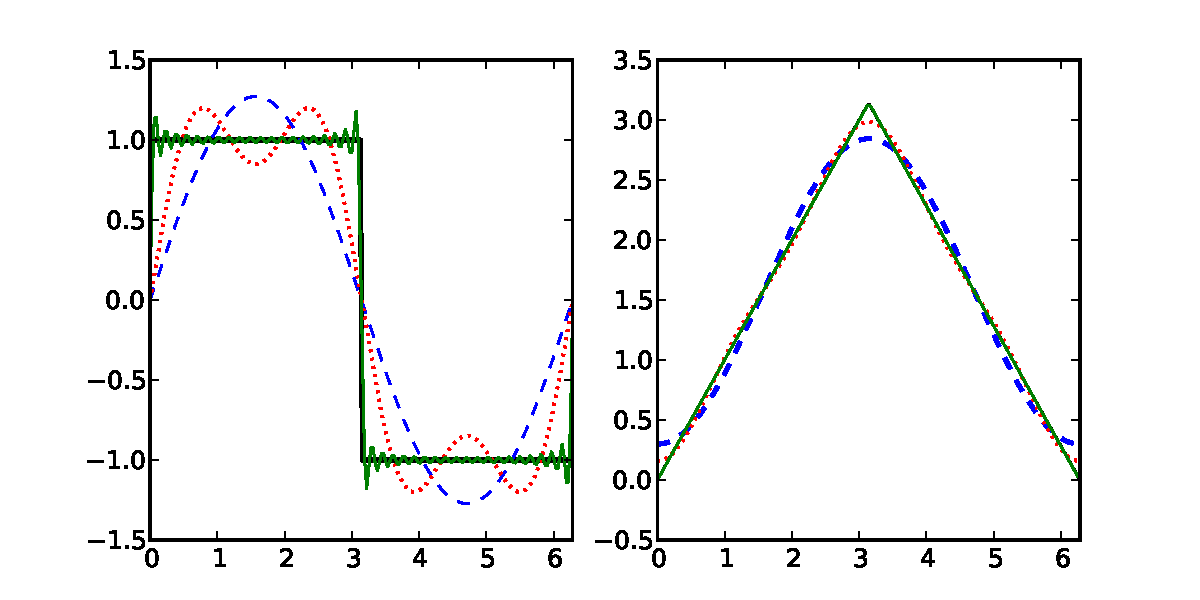
\includegraphics[width=\textwidth]{plots/fourier}
  \caption{Abgeschnittene Fourierreihen der Rechteckfunktion (links)
    und eines Dreeieckpulses (rechts). Die Funktionen sind jeweils als
    schwarze durchgezogene Linien eingezeichnet, die Näherungen mit
    einem Term blau gestrichelt, mit zwei Termen rot gepunktet, und
    mit 20 Termen grün durchgezogen. Für den Dreieckpuls ist letztere
    Näherung nicht mehr von der Funktion zu unterscheiden, während der
    Rechteckpuls noch deutliche Artefakte an den Unstetigkeiten zeigt.}
  \label{fig:fourier}
\end{figure}
Einige reelle Fourierreihen sind zum Beispiel:
\begin{itemize}
\item Konstante $f(t) = f_0$:
  \begin{equation}
    a_0 = 2 f_0,\quad a_n,\,b_n= 0\quad\text{sonst}
  \end{equation}
\item Rechteckfunktion
  \begin{equation}
    f(t) = \begin{cases}
      1 &\text{für}\; 0 \le t < \frac{T}{2} \\
      -1  &\text{für}\; \frac{T}{2} \le t < T
    \end{cases}\\
    = \quad\frac{4}{\pi}\sum_{n=1}^\infty
    \frac{1}{2n-1}\sin\left((2n-1)\omega t\right)
  \end{equation}
\item kurzer Rechteckpuls. Wir betrachten nun die auf konstanten
  Flächeninhalt normierte Funktion
  \begin{equation}
    f_S(t) = \begin{cases}
      1/S &\text{für}\; 0 \le t < S \\
      0  &\text{für}\; S \le t < T
    \end{cases},
  \end{equation}
  deren Fourierreihe
  \begin{equation}
    f_s(t) =
    \quad \frac{1}{T} +
    \quad\frac{2}{T}\sum_{n=1}^\infty
    \frac{\sin(n\omega S)}{n\omega S}\cos(n\omega t) +
    \frac{1-\cos(n\omega S)}{n\omega S}\sin(n\omega t)
  \end{equation}
  ist. Je kleiner $S$ wird und damit der Träger von $f_S$, desto
  langsamer konvergiert ihre Fourierreihe, da die Funktion $\sin(x)/x$
  immer dichter an der Null ausgewertet wird. Für jede feste Frequenz
  $n$ gilt schließlich
  \begin{equation}
    \widehat{\left(f_S\right)}_n \xrightarrow{S\to 0} \frac{1}{T} = \hat\delta_n
    \quad\text{für alle}\;n\in\ZZ
  \end{equation}
  bzw. $a_n\to 2/T$ und $b_n\to 0$. Die $\delta$-Funktion, die ja der
  formale Grenzwert der $f_S$ ist, und den kleinstmöglichen
  Träger hat, hat also in gewisser Weise die am schlechtesten
  (tatsächlich gar nicht!) konvergierende Fourierreihe.
\item Dreiecksfunktion
  \begin{equation}
    f(t) = \begin{cases}
      t      &\text{für}\; 0 \le t < \frac{T}{2} \\
      T - t  &\text{für}\; \frac{T}{2} \le t < T
    \end{cases}\quad=\quad\frac{\pi}{2} -
    \frac{4}{\pi}\sum_{n=1}^\infty
    \frac{1}{(2n-1)^2}\cos\left((2n-1)\omega t\right)
  \end{equation}
\end{itemize}
Genau wie die komplexe Fourierreihe lässt sich natürlich auch die
reelle Fourierreihe abschneiden, um Näherungen für Funktionen zu
bekommen, vergleiche Abbildung~\ref{fig:fourier}. Es fällt auf, das
die Fourierreihe besonders schlecht dort konvergieren, wo die Funktion
nicht differenzierbar ist bzw. einen Sprung aufweist.

\subsection{Diskrete Fouriertransformation}
\index{Fouriertransformation>diskrete}
\index{DFT}

\begin{figure}
  \centering
  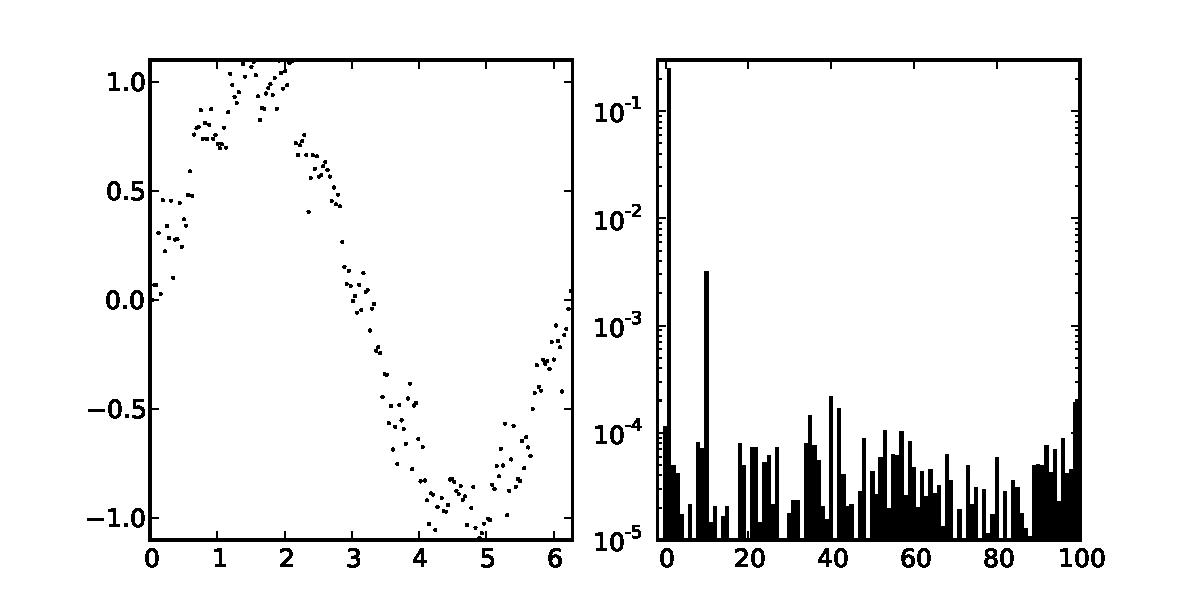
\includegraphics[width=\textwidth]{plots/fftsin}
  \caption{Diskrete Fouriertransformation von 200 diskreten
    Datenpunkten, die analog zu Abbildung~\ref{fig:leastsq} zwischen 0
    und $2\pi$ als $\sin(x) + 0,1\,sin(10 x) + \xi$ erzeugt wurden.
    Anders als der Funktionsfit erlaubt die DFT, auch die kleine
    zusätzliche Schwingung gut vom Rauschen zu unterscheiden. Im
    Graphen ist das Leistungsspektrum $\lvert DFT(k)\rvert^2$ gezeigt.
    Man erkennt die Amplitudenquadrate $0,25$ bei 1 und $0,01$ bei 10,
    auch wenn letztere Frequenz durch das Rauschen etwas an Intensität
    verloren hat.
  }
  \label{fig:fouriersin}
\end{figure}

\begin{figure}
  \centering
  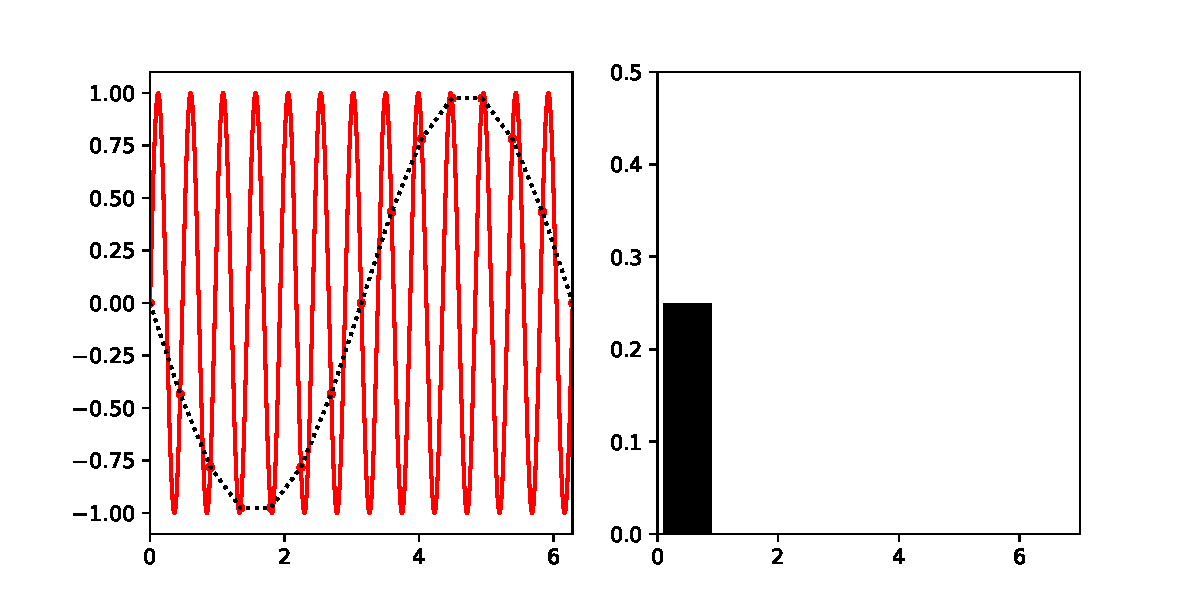
\includegraphics[width=\textwidth]{plots/fftalias}
  \caption{Diskrete Fouriertransformation von 14 äquidistanten
    diskreten Datenpunkten (rote Punkte links) der Funktion
    $\sin(13t)$ (rote Kurve links) im Interval $[0:2\pi]$.  Die
    Frequenz der Funktion $13/2\pi$ ist höher als die Nyquist-Frequenz
    $f_\text{Nyquist}=14/2\pi$, daher kommt es zu
    Aliasing-Artefakten. Die rekonstruierte Kurve ist links schwarz
    gepunktet eingezeichnet, ihr Spektrum rechts. Die abgetastete
    Funktion ist also scheinbar $\sin(t)$, was einer Frequenz von
    $2f_\text{Nyquist} - 13/2\pi$ entspricht.}
  \label{fig:fourieralias}
\end{figure}

Bei praktischen Anwendungen sind die Integrale zur Bestimmung der
Koeffiziente oft nicht analytisch lösbar, oder die Funktion ist von
vorneherein nur an diskreten Punkten gegeben, etwa weil es sich um
Messdaten handelt. In diesem Fall müssen die Integrale numerisch
approximiert werden. Wir betrachten nun also nicht mehr eine
kontinuierliche Funktion $f$, sondern Daten $f_k = f(t_k)$ mit
$t_k=k\Delta$, $k=0(1)N-1$ und Schrittweite $\Delta =
\frac{T}{N}$. Dann ist
\begin{equation}
  \hat{f}_n = \frac{1}{T}\int_0^T f(t)e^{-i n\omega t}\, dt
  \approx
  \frac{\Delta}{T}\sum_{k=0}^{N-1} f(k\Delta) e^{-i n\omega k\Delta}
  =
  \frac{1}{N}\sum_{k=0}^{N-1} f_k e^{-i\frac{2\pi}{N} n k} =: \frac{g_n}{N}.
\end{equation}
Die Koeffizienten
\begin{equation}
  \label{eq:dft}
  \text{DFT}(f_k)_n = g_n = \sum_{k=0}^{N-1} f_k e^{-i \frac{2\pi}{N} n k}
\end{equation}
werden als die \emph{diskrete Fouriertransformierte} bezeichnet, die
sehr effizient berechnet werden kann, wie wir im folgenden sehen
werden. Analog wird die \emph{inverse diskrete Fouriertransformation}
\begin{equation}
  \label{eq:idft}
  \text{iDFT}(g_n)_k = f(t_k) = \sum_{n=0}^{N-1} \frac{g_n}{N} e^{i \frac{2\pi}{N} n k}
\end{equation}
definiert, die aus den Koeffizienten wieder die Funktion $f$ an den
diskreten Eingangspunkten $t_k$
berechnet. Abbildung~\ref{fig:fouriersin} zeigt zum die DFT der Summe
zweier verrauschter Sinusfunktionen, aus der die beiden
Basisfrequenzen und deren Amplituden klar gegenüber dem Rauschen zu
erkennen sind.

Die Koeffizienten sind offenbar periodisch, da
\begin{equation}
  \label{eq:dftper}
  g_{n+N} = \sum_{k=0}^{N-1} f_k e^{-i\frac{2\pi}{N} (n + N) k} =
  \sum_{k=0}^{N-1} f_k e^{-i\frac{2\pi}{N} n k} \underbrace{e^{-2\pi i k}}_{=1} = g_n.
\end{equation}
Insbesondere ist $g_{-k} = g_{N-k}$, und es gibt nur $N$ echt
verschiedene Koeffizienten bzw. Frequenzen $n/T$. DFT-Bibliotheken
speichern die Koeffizienten daher meist als Vektor
$(g_{0},\ldots,g_{N-1})$
bzw. $(g_{0},\ldots,g_{N/2-1},g_{-N/2},\ldots,g_{-1})$.  Ist $f$
reell, so gilt noch dazu $g_{-k} = \overline{g_{k}}$, sodass lediglich
$\lceil N/2\rceil$ Koeffizienten wirklich verschieden sind. Allerdings
sind diese im allgemeinen komplex, so dass die $N$ reellen
Freiheitsgrade der Eingangsfunktion erhalten bleiben.

% verhindert zwei ziemlich unterfüllte Seiten
\enlargethispage{\baselineskip}

Die endliche Anzahl der diskreten Fourierkoeffizienten bedeutet, dass
bei einem reellen Signal mit Schrittweite $\Delta$ die maximal
darstellbare Frequenz $f_\text{Nyquist}=\frac{1}{2\Delta}$ beträgt,
die sogenannte
\emph{Nyquist-Frequenz}\index{Nyquist-Frequenz}. Signale mit höherer
Frequenz $f$ werden zu scheinbaren Signalen niedrigerer Frequenz
\begin{equation}
  f_\text{scheinbar} = \begin{cases}
    f \bmod 2 f_\text{Nyquist} & \text{falls}\; f \bmod 2 f_\text{Nyquist}
    < f_\text{Nyquist} \\
    2f_\text{Nyquist} - f \bmod 2 f_\text{Nyquist} & \text{falls}\; f \bmod 2 f_\text{Nyquist}
    \ge f_\text{Nyquist},
  \end{cases}
\end{equation}
was auch als \emph{Aliasing} bezeichnet
wird. Sollen analoge Signale digital weiter verarbeitet werden, kann
es daher notwendig sein, höhere Frequenzen durch analoge
Tiefpassfilter zu unterdrücken. Abbildung~\ref{fig:fourieralias}
illustriert dieses Problem.

\subsection{Schnelle Fouriertransformation}
\index{Fouriertransformation>schnelle}\index{FFT}

Die Berechnung der Fouriertransformierten nach \eqref{eq:dft} ist zwar
möglich, aber ziemlich langsam --- jeder der $N$ Koeffizienten
benötigt offenbar $\O(N)$ Operationen, so dass die DFT insgesamt
$\O(N^2)$ Operationen braucht. Das limitiert für praktische
Anwendungen $N$ auf einige tausend, was für viele Anwendungen zu wenig
ist. Die DFT konnte daher nur durch die \emph{schnelle
  Fouriertransformation} (FFT) von \emph{Cooley und Tukey} zu breiter
Anwendung finden. Diese basiert auf der Beobachtung, dass für $N=2M$
\begin{align}
  \text{DFT}(f_k)_n &= \sum_{k=0}^{M-1} f_{2k} e^{-i\frac{2\pi}{2M} n\, 2k} +
  \sum_{k=0}^{M-1} f_{2k+1} e^{-i\frac{2\pi}{2M} n\, (2k + 1)}\\
  &= \text{DFT}(f_{2k})_n + e^{-i\frac{2\pi}{2M} n}
  \text{DFT}(f_{2k+1})_n,
\end{align}
wobei $\text{DFT}(f_{2k})_n$ den $n$-ten Koeffizienten einer DFT auf
den Datenpunkten $f_{2k}$, $k=0(1)M-1$, bezeichnet. Gemäß
\eqref{eq:dftper} ist dabei $\text{DFT}(f_{2k})_n =
\text{DFT}(f_{2k})_{n-M}$ für $n>M$.

Die Fouriertransformatierte der $N$ Datenpunkte ergibt sich also als
einfache Summe von zwei
Fouriertransformierten mit lediglich der halben Menge $M$ an
Datenpunkten, wobei die ungerade Hälfte mit der \emph{Einheitswurzel}
\begin{equation}
  w^n := e^{-i\frac{2\pi}{2M} n}
\end{equation}
multipliziert wird.  Ist nun $M$ wieder durch zwei teilbar, so lassen
sich diese Fouriertransformierten ebenfalls als Summe zweier nochmals
halb so langer Fouriertransformationen darstellen. Wenn nun $N$ eine
Zweierpotenz ist, kann man so fortfahren, bis $M=1$ erreicht ist, also
$\text{DFT}(f_0)_0 = f_0$. Dabei gibt es offenbar $\log_2(N)$ viele
Unterteilungsschritte, die jeder $\O(N)$ Operationen kosten. Insgesamt
benötigt die FFT also lediglich $\O(N\log N)$ Operationen.

Schematisch funktioniert ein FFT-Schritt wie folgt:
\begin{center}
  \begin{tikzpicture}[x=2em,y=3em,>=stealth']
    \draw (0,0)  node (f0) {$f(0)$} ;
    \draw (0,-1) node (f1) {$f(\Delta)$} ;
    \draw (0,-2) node (f2) {$f(2\Delta)$} ;
    \draw (0,-3) node (f3) {$f(3\Delta)$} ;

    \draw (3,0.25) rectangle +(2,-1.5);
    \draw (4,-0.5) node {
      \begin{minipage}{4em}\centering
        Halbe\\
        FFT
      \end{minipage}
    } ;

    \draw (3,-1.75) rectangle +(2,-1.5);
    \draw (4,-2.5) node {
      \begin{minipage}{4em}\centering
        Halbe\\
        FFT
      \end{minipage}
    } ;

    \draw (8,0)  node (g0) {$g_0$} ;
    \draw (8,-1) node (g1) {$g_1$} ;
    \draw (8,-2) node (g2) {$g_2$} ;
    \draw (8,-3) node (g3) {$g_3$} ;

    \draw[->] (f0) -- (3,0);
    \draw[->] (f2) -- (3,-1);
    \draw[->] (f1) -- (3,-2);
    \draw[->] (f3) -- (3,-3);

    \draw[->] (5,0)   -- node[above,pos=0.97] {$\cdot 1$} (g0.west);
    \draw[->] (5,-2)  -- node[below,pos=0.97] {$\cdot w^0$}(g0.west);
    \draw[->] (5,-1)  -- node[above,pos=0.97] {$\cdot 1$}(g1.west);
    \draw[->] (5,-3)  -- node[below,pos=0.97] {$\cdot w^1$}(g1.west);
    \draw[->] (5,-2)  -- node[above,pos=0.97] {$\cdot 1$}(g2.west);
    \draw[->] (5,0)   -- node[below,pos=0.97] {$\cdot w^2$}(g2.west);
    \draw[->] (5,-3)  -- node[above,pos=0.97] {$\cdot 1$}(g3.west);
    \draw[->] (5,-1)  -- node[below,pos=0.97] {$\cdot w^3$}(g3.west);
  \end{tikzpicture}
\end{center}
Aufgrund ihres Aussehens wird dieses Datenpfadschema auch als
Butterfly-Schema genannt. Damit die beiden Unter-FFTs auf einem
zusammenhängenden Satz von Daten operieren können, müssen also auch
die Eingabedaten $f_k$ umsortiert werden, ebenso wie auch für die
Unter-FFTs. Man kann sich leicht überlegen, dass dabei $f_k$ auf
$f_{k'}$ sortiert wird, wobei die Bits  $k'$ in Binärdarstellung
dieselben wie von $k$ sind, nur in umgedrehter Reihenfolge.

Die FFT erlaubt also die effiziente Zerlegung einer Funktion in ihre
Schwingungskomponenten, was viele wichtige Anwendungen nicht nur in
der Physik hat. Daher gibt es eine Reihe sehr guter Implementierungen
der FFT, allen voran die "`Fastest Fourier Transform in the West"'
(FFTW, \url{http://www.fftw.org}). Selbstverständlich bietet auch NumPy
eine FFT, \scipy{numpy.fft.fft(f_k)}, mit der inversen FFT
\scipy{numpy.fft.ifft(g_n)}. Die Routinen sind so implementiert, dass
bis auf Maschinengenauigkeit $\text{iFFT}(\text{FFT}(f_k)) = f_k$.

Wichtige Anwendungsbeispiele der diskreten Fouriertransformation sind
zum Beispiel die Datenformate JPEG, MPEG und MP3, die alle drei auf
einer Abwandlung der DFT beruhen, der \emph{diskreten
  Cosinustransformation} (DCT) für reelle Daten. Bei dieser wird der
Datensatz so in der Zeitdomäne verdoppelt, dass er in jedem Fall eine
gerade Funktion repräsentiert, wodurch die Fourierreihe in eine reine
Cosinusreihe übergeht mit nur reellen Koeffizienten. Die DCT ist also
eine Umwandlung reeller in reelle Zahlen. Wegen Ihrer Wichtigkeit gibt
es nicht nur extrem effiziente Implementierungen für die meisten
Prozessortypen, sondern auch spezielle Hardware.

\section{\keyword{Wavelets}}
\index{Multiskalenanalyse}

Die Fouriertransformation wird vor allem deshalb für die Kompression
von Audio- oder Bilddaten genutzt, weil sie hochfrequente von
niederfrequenten Signalen trennt und die menschlichen Sinne die
hochfrequenten Anteil meist nicht gut wahrnehmen können. Das ist
allerdings nicht ganz korrekt, tatsächlich können wir nur stark lokale
Änderungen nicht gut wahrnehmen. Dafür sind Fourierreihen an sich gar
nicht so gut geeignet, da ja auch die hochfrequenten Schwingungen
alles andere als lokal sind. Als Alternative hat sich die
\emph{Multiskalenanalyse} (MSA) oder \emph{diskrete
  Wavelettransformation} etabliert, die auch im transformierten Raum
lokal ist.

\begin{figure}
  \centering
  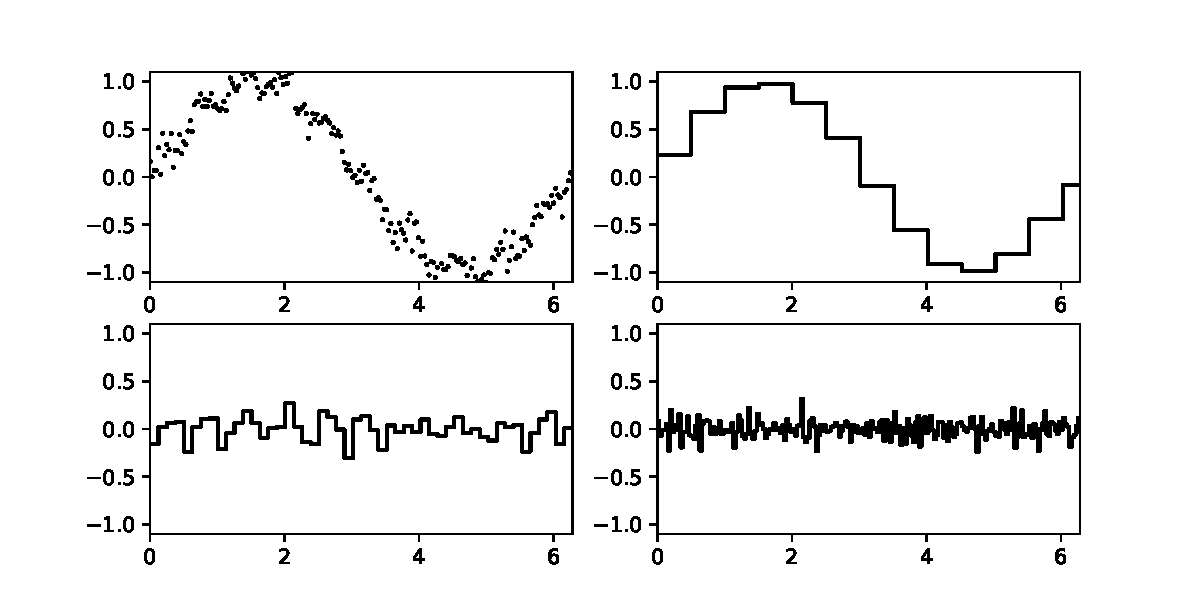
\includegraphics[width=\textwidth]{plots/wavelet}
  \caption{Diskrete Wavelettransformation von 200 diskreten
    Datenpunkten, die analog zu Abbildung~\ref{fig:fouriersin} zwischen
    0 und $2\pi$ als $\sin(x) + 0,1\,sin(10 x) + \xi$ erzeugt
    wurden. Für die Transformation wurden die Wavelets von $(0,1]$ auf
    den Bereich $(0,2\pi]$ gestreckt. Der linke obere Graph zeigt
    nochmals das Ausgangssignal, von rechts oben nach rechts unten
    folgen die Anteile der Stufen 0--3, also $(f,\phi_0)\phi_0 +
    \sum_{j=0}^{3} \sum_{k=0}^{2^j-1} (f,\psi_{jk})\psi_{jk}$, dann
    Stufen 4 und 5 ($\sum_{j=4}^{5} \sum_{k=0}^{2^j-1}
    (f,\psi_{jk})\psi_{jk}$) und schließlich Stufen 6--8, womit die
    Auflösung der Ausgangsdaten erreicht ist.}
  \label{fig:dwt}
\end{figure}

Anders als bei der Fouriertransformation, die eine Zerlegung in
trigonometrische Funktionen darstellt, gibt es für die MSA
verschiedene Sätze von Basisfunktionen mit verschiedenen Eigenschaften
wie Differenzierbarkeit und Lokalität. Im folgenden soll die MSA mit
Hilfe des Haar-Wavelets dargestellt werden, dass das einfachste und
älteste bekannte Wavelet ist. Zunächste betrachten wir die
\emph{Skalierungsfunktion}
\begin{equation}
  \phi(x) = \chi_{(0,1]} =
  \begin{cases}
    1 &\text{für}\; 0 < x \le 1\\
    0 &\text{sonst}
  \end{cases}
\end{equation}
sowie das Haar-\emph{Wavelet}
\begin{equation}
  \psi(x) =
  \begin{cases}
    -1 &\text{für}\; 0 < x \le \frac{1}{2}\\
    1 &\text{für}\; \frac{1}{2} < x \le 1 \\
    0 &\text{sonst},
  \end{cases}
\end{equation}
aus denen wir die Basisfunktionen $\phi_k(x) := \phi(x - k)$ der nullten
Stufe und $\psi_{jk}(x) := 2^{j/2}\psi(2^jx-k)$ der $j$-ten Stufe
konstruieren. Durch die Skalierung mit $2^j$ werden die $\psi_{j,k}$
also immer schmaler, sind aber wegen des Vorfaktors alle normiert,
d.h. $\lVert \psi_{jk} \rVert = 1$. Ebenso sind auch die $\phi_k$
normiert. Zusätzlich sind sämtliche Basisfunktionen zu einander
orthogonal, wie man sich leicht überlegt. Daher lässt sich jede
quadratintegrable Funktion $f$ wie folgt zerlegen:
\begin{equation}
  f(x) = \sum_{k\in\ZZ} (f,\phi_k)\phi_k + \sum_{j\in\NN_0}
  \sum_{k\in\ZZ} (f,\psi_{jk})\psi_{jk}
\end{equation}
Dies ist die Multiskalenanalyse von $f$. Die Koeffizienten der Stufe
$j$ werden auch Details der Stufe $j$ genannt. In der Praxis ist das
Signal durch endlich viele äquidistante Datenpunkte gegeben, analog
zur diskreten Fouriertransformation. In diesem Fall sind die Summen
endlich, da einerseits der Träger endlich ist und damit nur endlich
viele $(f,\phi_k)\neq 0$, und es andererseits keine Details unterhalb
der Auflösung des Signals gibt. Man skaliert dann die Wavelets und
Skalierungsfunktion so, dass der Abstand der Datenpunkte gerade der
halben Breite des Wavelets auf der feinsten Auflösung entspricht, und
$\phi = \phi_0$ bereits das gesamte Interval überdeckt. Für eine nur
auf $[0,1]$ nichtverschwindende Funktion, deren Werte an $2^N$ Punkten
äquidistanten Punkten bekannt ist, reduziert sich die
Multiskalenanalyse zur \emph{diskreten
  Wavelettransformation}\index{Wavelets>-transformation}
\begin{equation}
  \label{eq:idwt}
  f(x) = (f,\phi)\phi +
  \sum_{j=0}^{N-1} \sum_{k=0}^{2^j-1} (f,\psi_{jk})\psi_{jk}.
\end{equation}
Die Anzahl der Koeffizienten ist dann $1 + 1 + 2 + \cdots + 2^{N-1} =
2^N$, also genau die Anzahl der Eingabedaten. Genau wie die diskrete
Fouriertransformation bildet die Wavelettransformation $2^N$ Werte
$f(k/2^N)$ auf $2^N$ Werte $(f,\phi)$ und $(f,\psi_{jk})$ ab und
besitzt eine exakte Rücktransformation, \eqref{eq:idwt}.

Analog zur schnellen Fouriertransformation gibt es auch eine schnelle
Wavelettransformation (FWT), die sogar linearen Aufwand hat, also $\O(N)$
Schritte bei $N$ Datenpunkten benötigt. Eine einfache Implementation
der FWT und der inversen FWT für das Haar-Wavelet zeigt
Codebeispiel~\ref{lst:dwt}. Der Kern dieser Transformation liegt
darin, die Transformierte von der höchsten Detailauflösung herab
aufzubauen, und dadurch die die Integrale approximierenden Summen
schrittweise aufzubauen (\emph{Downsampling}). Für genauere
Informationen siehe zum Bespiel \textcite{daubechies92a}.

Abbildung~\ref{fig:dwt} zeigt einige Detailstufen der
Wavelet-Zerlegung der verrauschten Sinusfunktionen analog
Abbildung~\ref{fig:fouriersin}. Auch hier lässt sich das Rauschen auf
den höheren Detailstufen gut vom Nutzsignal trennen, allerdings kann
die Oberschwingung nicht detektiert werden. Das hängt allerdings vor
allem daran, dass das Haar-Wavelet nicht sehr geeignet ist, da es
nicht glatt ist, im Gegensatz zum Nutzsignal. Daher sind in den
meisten Fällen glatte Wavelets besser geeignet. Das bekannteste
Beispiel von glatten Wavelets sind die Daubechies-Wavelets, die
daneben auch einen kompakten Träger haben, also stark lokalisiert
sind. Mit solchen Wavelets lassen sich sogar reale Musikdaten in
Akkorde zurücktransformieren. Auch der JPEG-Nachfolger JPEG2000
basiert auf einer Wavelettransformation statt einer
Cosinustransformation, allerdings mit
Cohen-Daubechies-Feauveau-Wavelets.

\lstinputlisting[style=floating,
caption={Diskrete Wavelettransformation und ihre Inverse als
  Python-Code. Die Länge der Eingabedaten muss eine Zweierpotenz $2^N$
  sein. Die Details sind in einem Vektor $c$ gespeichert, in der Form
  $c=((f,\phi_0)$, $(f, \psi_{00})$, $(f, \psi_{10})$, $(f, \psi_{11})$,
  $(f, \psi_{20})$, $(f, \psi_{21})$, $(f, \psi_{22}), \ldots,
  (f, \psi_{N-1,2^{N-1}-1}))$.
},
label=lst:dwt]{dwt.py}

%%% Local Variables: 
%%% mode: latex
%%% TeX-master: "padc"
%%% TeX-PDF-mode: t
%%% End: 
